% Pour guider la définition de notre méthode nous avons identifié
% plusieurs principes que nous voulons voir respectés.

\subsection{Intégration dans le contexte métier}

Le premier des principes que nous voulons voir respecté par notre
méthodologie est celui de sa bonne intégration dans le contexte
métier.
%
C'est un point que nous avons déjà évoqué a plusieurs reprises. Nous
souhaitons que notre méthode soit conçue dans l'optique de son
application finale, \ie que nous avons à cœur de réfléchir à son
appropriation et son développement par les secouristes. Pour autant
nous ne souhaitons pas sacrifier la généricité de notre méthode, c'est
pourquoi son développement relève d'un équilibre entre la généricité
de la méthode et la spécificité de certains paramétrages.

\subsubsection{Prérequis nécessaires à la méthode de construction
  d'une zone de localisation probable}
\label{sec:4-1-1-1}

Comme nous l'indiquions dans la première partie, un des partis-pris
fondamentaux du projet CHOUCAS est d'intégrer pleinement les
secouristes au processus de localisation de la victime, ce qui impose
le développement de solutions d'aide à la décision et non
d'automatisation de la localisation. Si ce choix n'appose pas de
contraintes spécifiques sur nos travaux, il nous offre des
possibilités inédites. En effet, ce parti-pris impose la présence
constante d'un secouriste, en contact avec le requérant et
interagissant avec notre méthode de localisation par le biais de
l'interface développée au sein du projet Choucas
(\ref{subsec:1-2-3-3}). Par conséquent, nous pouvons développer une
méthode nécessitant la participation active d'un secouriste lors de
son application.

Nous avons donc décidé de compter sur les secouristes pour construire
les \emph{indices de localisation} à partir des informations données
par le requérant. Cette opération consiste à identifier les différents
élément constituant \emph{l'indice de localisation} (\emph{sujet,}
\emph{objet de référence,} \emph{relation de localisation}) dans le
discours du requérant, puis de les renseigner dans l'interface. Ce
travail ne se résume cependant pas à une opération de saisie et impose
également un travail d'analyse et de désambiguïsation du discours du
requérant. Pour l'illustrer prenons l'exemple de la phrase :
\enquote{Je suis à deux pas d'une maison}. La première tâche que nous
confions au secouriste est celle de l'identification des éléments de
la phrase, \enquote{je} est le \emph{sujet,} \enquote{à deux pas} est
une \emph{relation de localisation} et \enquote{une maison} est
\emph{l'objet de référence.} Mais cette segmentation ne suffit pas à
\emph{spatialiser} cet \emph{indice de localisation.} Pour ce faire il
est nécessaire d'interpréter ces trois chaines de caractères pour
identifier l'objet ou le concept auquel elles se référent. Dans le cas
d'une automatisation intégrale il serait nécessaire de définir une
méthode à cet effet, mais nous pouvons déléguer cette tâche au
secouriste. La \emph{relation de localisation} \enquote{à deux pas}
peut, par exemple, être considérée comme une \emph{relation de
  distance métrique quantitative} (cf. \ref{sec:3-1-dist_met_quant}),
pourtant on peut supposer que la notion centrale de cet exemple est la
notion de \emph{proximité} est non une quantification de
distance. L'automatisation de ce travail de désambiguïsation est
extrêmement difficile et est un champ de recherche spécifique, c'est
pourquoi nous le déléguons au secouriste. Dans les faits cela implique
que c'est à ce dernier de choisir la \emph{relation spatiale,} à
partir d'une liste prédéfinie, en fonction du contexte et de sa
compréhension de \emph{l'indice de localisation}. Ainsi, pour
reprendre l'exemple précédent, c'est au secouriste de choisir si la
\emph{relation de localisation} \enquote{à deux pas} doit être
modélisée comme une relation de \emph{proximité} où une \emph{distance
  métrique quantitative.}

De manière analogue il revient au secouriste d'analyser l'objet de
référence. Dans notre exemple, \emph{l'objet de référence}
(\enquote{une maison}) désigne un type d'objet (\ie un \emph{géotype})
auquel plusieurs objets (\ie les \emph{géons}) peuvent
correspondre. Ce travail d'identification des objets géographiques
utilisés comme référence par le requérant peut également être délégué
au secouriste, par le biais de l'interface. Pour notre exemple le
secouriste devra sélectionner tous les objets correspondant à la
description donnée par le secouriste. Cette approche pose néanmoins un
problème, celui de l'aire de la sélection. En effet, sans information
supplémentaire tout objet géographique correspondant à la sélection
peut être considéré comme un objet de référence valide. Il est donc
nécessaire de définir une \emph{zone de travail} délimitant l'aire de
recherche de la victime, et par conséquent de sélection des
\emph{objets de référence.} Dans l'ontologie d'alerte CHOUCAS (OAC,
\cite{Viry2019}), cette région est qualifiée de \emph{zone initiale de
  recherche} (ZIR). La définition d'une telle zone est un préalable
indispensable à la \emph{spatialisation} des \emph{indices de
  localisation.}

Ainsi, notre méthodologie impose trois tâches au secouriste. La
première, effectuée au début de la phase de localisation, consiste à
définir la ZIR. La seconde consiste à identifier, à partir d'une liste
préalablement définir, \emph{la relation de localisation}
correspondant au mieux à \emph{l'indice de localisation,} puis, le
secouriste doit sélectionner les \emph{objets de référence} utilisés
par le requérant.
%
Ainsi, en entrée de notre méthode nous disposons, pour chaque
\emph{indice de localisation} d'une \emph{relation de localisation}
exprimée dans un vocabulaire contrôlé et d'un ensemble d'objets
géographiques, servant de référence.


% \tdi{Ajout figure diag activ secours}
% \begin{figure}
%   \centering
%   % \input{../figures/diag_activ_secours.tex}
%   \caption{dcsqd}
%   \label{fig:diag_acti_secours}
% \end{figure}

\subsubsection{La modélisation explicite des connaissances}

Les phases de \emph{spatialisation} et de \emph{fusion} différent par
un point essentiel. La fusion consiste à regrouper différentes
\emph{zones de localisation compatibles} dans le but de construire une
seule \emph{zone de localisation probable} \footnote{Bien qu'elle
  puisse être discontinue.}, par conséquent, tous les individus
fusionnés sont de même nature, ce sont des objets géographiques. Une
même méthode peut donc être employée dans toutes les configurations,
qu'il soit nécessaire de fusionner deux \emph{zones de localisation}
identiques ou trente \emph{zones} extrêmement différentes. Cette
généricité n'est cependant pas partagée par la méthode de
\emph{spatialisation,} qui doit avoir un comportement adapté à la
chaque \emph{relation de localisation.} En effet, on ne peut
spatialiser la \emph{relation} \enquote{sous} de la même manière que
les \emph{relations} \enquote{entre} ou \enquote{proche}. Il est donc
nécessaire de définir (et d'implémenter) une méthode de
\emph{spatialisation} pour toutes les \emph{relations de localisation}
traitées. Ces différentes méthodes de \emph{spatialisation} sont d'une
grande importance. D'une part, car elles constituent le cœur de notre
travail de développement, c'est par elles qu'une description de
position devient une \emph{zone de localisation compatible,} de
l'autre, car l'implémentation de ces méthodes devient \emph{de facto}
un cadre formel, fixant ---~par le biais de leur
\emph{spatialisation}~--- la sémantique que nous attribuons à chaque
\emph{relation de localisation.} Pour le dire autrement, la meilleure
façon de comprendre comment est traitée une \emph{relation de
  localisation} donnée est de consulter le code qui se destine à la
\emph{spatialiser.} Ce faisant l'ensemble des connaissances produites
lors de l'élaboration des méthodes de \emph{spatialisation} serait
principalement sous forme de code, ce qui est une limite forte à la
compréhension et l'utilisation appliquée de notre travail, en plus de
s'opposer au principe \emph{d'intégration dans le contexte métier.}

Nous avons donc cherché à séparer autant que possible la formalisation
de la sémantique des \emph{relations de localisation} de leur
implémentation, en adoptant une démarche de la modélisation explicite
des connaissances, librement inspirée des \emph{systèmes à base de
  connaissances} \todo{Citer
  \url{https://hal.inria.fr/inria-00201566/document}}. Dans ces
systèmes, les connaissances sont formalisées au sein d'une ontologie
lue et interprétée par un logiciel. On peut donc imaginer que les
règles de \emph{spatialisation} de toutes les \emph{relations de
  localisations} soient formalisées dans une ontologie \emph{ad hoc}
et interprétées et appliquées par un logiciel spécifique. Cette
approche a de multiples avantages, d'une part, elle permet aux
utilisateurs des méthodes de \emph{spatialisation} de disposer d'une
forme d'auto-documentation, permise par la centralisation de toutes
les règles de \emph{spatialisation.} De plus, cette centralisation
facilite également la modification où l'ajout de règles de
\emph{spatialisation,} faisant de l'ontologie un outil facilitant
l'amélioration des méthodes de \emph{spatialisation.} Enfin, le cadre
formel et la centralisation offerts par l’utilisation d'une ontologie
facilite la diffusion de notre travail, un tel document pouvant être
plus facilement étudié, voire réutilisé, qu'un code informatique, même
diffusé librement.

\subsection{Principes de modélisation}

\subsubsection{Décomposition des \emph{relations de localisation}}

Comme nous l'avons déjà indiqué (\autoref{subsec:2-1-1}), une même
\emph{relation de localisation} peut avoir une sémantique différente
en fonction de son contexte d'utilisation
\autocite[16]{Borillo1998}. Par exemple, la \emph{relation de
  localisation} \enquote{\emph{sous}} n'a pas exactement la même
signification dans les phrases : \enquote{Je suis sous \emph{un pont}}
et \enquote{Je suis sous \emph{une route}}. La première phrase
sous-entend une idée de \emph{recouvrement} (\ie \emph{le pont est
  entre le locuteur et le ciel}), que l'on retrouve également dans
l'expression imagée \enquote{Je suis sous l'eau}, mais cette notion
est absente dans la seconde phrase, qui décrit une configuration où le
recouvrement est impossible. Il est intéressant de noter l'intuitivité
\footnote{Dans la mesure où l'on est un locuteur humain.} de cette
distinction. De fait, on comprend immédiatement que la phrase
\enquote{Je suis sous un pont} décrit une configuration plus précise
qu'une simple différence d'altitude et, à l'inverse, on ne peut
imaginer que la phrase : \enquote{Je suis sous une route} décrive une
situation où le locuteur est littéralement recouvert par la
voirie. Cette interprétation différente de deux phrases très
similaires ne s'explique que par leur point divergent, leur
\emph{objet de référence} et plus particulièrement, leur nature. On
peut, en effet, être recouvert par \emph{un pont} (ou un arbre, une
table, le ciel, \emph{etc.}) mais pas par une route (ou un
glacier). \emph{L'objet de référence} et plus généralement le contexte
d'utilisation d'une \emph{relation de localisation,} peut donc influer
sa signification. Dès lors, on ne peut prétendre spatialiser des
\emph{relations de localisation} sans être capable d'identifier ces
variations de sémantique, leurs causes et leurs conséquences.

On peut aborder ce problème en postulant que la différence sémantique
de ces deux exemples s'explique en réalité par l’emploi de deux
\emph{relations de localisations} différentes, mais désignées par la
même \emph{préposition spatiale :} \enquote{sous}. Adopter cette
vision implique donc de considérer que le \enquote{sous} \emph{avec
  recouvrement} est une \emph{relation de localisation} différente du
\enquote{sous} \emph{sans recouvrement} et ce bien qu'elles soient
exprimées avec la même \emph{préposition spatiale.} Une manière
alternative d'illustrer ce postulat est de le généraliser à l'ensemble
du vocabulaire. Ainsi, on pourrait considérer que les différentes
définitions d'un même mot, que l'on peut trouver dans un dictionnaire,
définissent des concepts différents, mais exprimés avec le même
mot. Cette conception a beau présenter un certain intérêt
intellectuel, elle n'apporte pas réellement de solutions. D'une part
elle ne dispense pas du travail d’identification des variantes des
\emph{relations de localisation,} mais quelle approche le pourrait ?
De l'autre, elle ignore un élément important que nous n'avons pas
encore mentionné, les \emph{récurrences sémantiques.} Si le
\enquote{sous} avec et sans recouvrement s'opposent, ils partagent une
part importante de leur sémantique, ce qui leur vaut d'être désignés
avec la même préposition. Ces deux \emph{relations} traduisent toutes
deux une situation ou le \emph{sujet} a une altitude inférieure à
\emph{l'objet de référence} et où ces deux éléments ne sont pas très
éloignés. La notion de recouvrement ne fait que s'ajouter à ces deux
notions. Aussi, ces deux \enquote{sous} ont plus de points communs que
de points de divergence. On observe donc la présence de
\emph{récurrences sémantiques} entre ces deux \emph{relations.} On
peut tirer parti de ces récurrences pour améliorer notre précédent
postulat. Ainsi, on peut considérer que les deux variantes du
\enquote{sous} sont des \emph{relations de localisation} différentes
car elles combinent des \enquote{briques sémantiques} différentes,
tout en partageant la plupart. L’intérêt majeur de ce point de vue
c'est qu'il laisse entrevoir une possibilité, celle d'exploiter ces
récurrences sémantiques pour la \emph{spatialisation}
\autocite{Bunel2019a}. Pour ce faire, nous proposons
\enquote{d'extraire}, lors d'un processus que nous appelons
\emph{décomposition,} ces \enquote{briques sémantiques} des
\emph{relations de localisation,} pour définir un ensemble de
\emph{relations de localisation atomiques,} qui, combinées recréent la
sémantique de la \emph{relation de localisation} décomposée. La mise
en place de cette approche nécessite l'identification et
l'explicitation préalables des \emph{relations de localisation
  atomiques,} conformément au \emph{principe de modélisation explicite
  des connaissances.} Chaque relation de \emph{localisation atomique}
correspondant alors à une composante sémantique indépendante.

Pour illustrer cette démarche on peut l'appliquer à \emph{l'indice de
  localisation} : \enquote{Je suis sous une route}. Comme nous l'avons
mentionné, la \emph{relation de localisation} utilisée décrit ici une
situation où le locuteur est situé à une altitude inférieure d'une
route donnée, mais également a proximité de cette dernière, de sorte a
ce que la relation de verticalité entre le locuteur et la route soit
saillante \autocite{Vandeloise1986}. La relation de localisation
\enquote{sous} peut ici être décomposée en deux \emph{relations de
  localisation atomiques,} la première indiquant que le \emph{sujet}
est situé plus bas que \emph{l'objet de référence} et la seconde
indiquant qu'il en est proche.

La \emph{décomposition} de la \emph{relation de localisation} conduit
à construire deux nouveaux \emph{indices de localisation,} qui ne
diffèrent que par leur \emph{relation de localisation.} On peut alors
\emph{spatialiser} \emph{l'indice de localisation} en combinant les
\emph{spatialisations} des \emph{relations de localisations
  atomiques.} Par exemple, si l'on cherche à modéliser l'\emph{indice
  de localisation} \enquote{je \emph{suis sous} un pont} on pourra
construire la \emph{zone de localisation} correspondant à
\emph{l'indice de localisation} \enquote{je suis \emph{recouvert} par
  un pont} et la \emph{zone de localisation} correspondant à
\emph{l'indice de localisation} \enquote{je suis \emph{à une altitude
    inférieure} à un pont}, puis les combiner à l'aide d'un opérateur
de fusion \emph{ad hoc,} pour obtenir la \emph{zone de localisation
  compatible} correspondant à \emph{l'indice de localisation}
\enquote{je suis \emph{sous} un pont}.

Cette approche a pour objectif et intérêt principal de permettre
l'exploitation des récurrences sémantiques que l'on peut trouver entre
différentes \emph{relations de localisation.} Par exemple, la notion
de \emph{proximité} est à la base de nombreuses \emph{relations de
  localisation} comme \enquote{\emph{à côté}}, \enquote{\emph{aux
    alentours de}}, \enquote{\emph{devant}}, \emph{etc.} En
définissant une méthode de \emph{spatialisation} de cette
\emph{relation de localisation atomique} il devient possible de la
réutiliser et de la combiner à d'autres \emph{relations de
  localisation atomiques} permettant ainsi de modéliser un grand
ensemble de \emph{relations de localisations.}

On peut cependant s'attendre à ce que plusieurs \emph{relations de
  localisation} ne soient pas décomposables en un ensemble de
\emph{relations de localisation atomiques.} C'est par exemple le cas
de la notion de \emph{proximité} qui peut être employée
indépendamment, comme dans la phrase \enquote{je suis proche d'un
  supermarché}. Ainsi certaines \emph{relations de localisation} sont
des \emph{relations atomiques,} non décomposables.

%\tdi{Ajouter le principe de décomposition des objets ?}

\subsubsection{Autonomie de la \emph{spatialisation}}

Un autre principe que nous souhaitons développer est celui de la
séparation maximale des étapes du processus.

Comme nous l'expliquions dans le \autoref{chap:02} deux étapes sont
nécessaires pour transformer une position décrite en une \emph{zone de
  localisation probable,} la \emph{spatialisation} et la
\emph{fusion.} Mais ces deux étapes peuvent être combinées
différemment.

Une première solution consiste à \enquote{chainer} la
\emph{spatialisation} des différents \emph{indices de localisation,}
comme on peut le voir sur la figure \ref{fig:comp_approches_lin}. Avec
cette approche les différentes \emph{zones de localisation
  compatibles} sont créées les unes à la suite des autres, ainsi la
zone de recherche en entrée de chaque étape de \emph{spatialisation}
dépend des \emph{spatialisations} précédentes. Avec cette approche,
l'opération de \emph{fusion} est implicite, elle s'opère, en partie, à
chaque nouvelle \emph{spatialisation,} puisque les zones ne
correspondant pas aux \emph{indices de localisation} sont retirées peu
à peu. La \emph{zone de localisation probable} (en bleu sur la figure
\ref{fig:comp_approches}) est obtenue une fois que l'on a
\emph{spatialisé} tous les \emph{indices de localisation.} Cette
approche est la première que nous ayons envisagée. Elle a pour
avantage d'être simple à concevoir et à développer. Cependant cette
approche à un problème majeur. À cause de l'enchainement des étapes de
\emph{spatialisation} les erreurs se répercutent d'une étape à
l'autre. Ainsi, si un des \emph{indices de localisation} est mal
\emph{spatialisé}, que ce soit à cause de la méthode utilisée ou d'une
mauvaise description, cela se répercute sur toutes les
\emph{spatialisations} ultérieures. La moindre correction impose donc
de refaire l'ensemble des traitements.

Une seconde solution, plus robuste, consiste à effectuer l'ensemble
des opérations de \emph{spatialisation} en parallèle, comme le montre
la figure \ref{fig:comp_approches_sep}. Avec cette approche la
\emph{spatialisation} des différents \emph{indices de localisation}
est effectuée séparément et leur \emph{fusion} est effectuée dans un
second temps. Comme pour la démarche \enquote{chainée} une
\emph{spatialisation} erronée peut impacter la \emph{zone de
  localisation probable,} toutefois il est plus facile de corriger ces
erreurs. En effet, si les différentes \emph{zones de localisation
  compatibles} ont été conservées il est possible de faire une
nouvelle \emph{fusion} en retirant un, ou plusieurs \emph{indices de
  localisation.} Alors qu'avec une approche \enquote{chainée} il est
nécessaire de refaire toutes les opérations de \emph{spatialisations}
ultérieures à celle de \emph{l'indice de localisation} que l'on
souhaite modifier ou retirer et ce même si les résultats
intermédiaires ont été conservés.

\begin{figure}
  \centering
  \subfloat[Construction suivant une démarche linéaire]{
    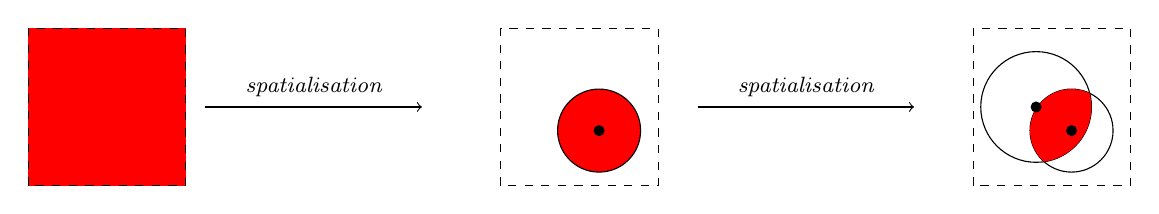
\begin{tikzpicture}

  \begin{scope}
    \path[fill=red] (0,0) rectangle (2,2);
	\path[draw, dashed] (0,0) rectangle (2,2);
  \end{scope}

  \path[draw, ->] (2.25,1) --++ (2.75,0)  node[pos=.5, above] {\footnotesize \itshape spatialisation};

  \begin{scope}[xshift=6cm]
	\path[draw, dashed] (0,0) rectangle (2,2);
	\begin{scope}
	    \begin{scope}
	      \clip (0,0) rectangle (2,2);
	      \fill[red] (1.25,.7) circle [radius=15pt];
	      \path[draw] (1.25,.7) circle [radius=15pt];
	    \end{scope}
	\end{scope}
    \node[circle, inner sep=0pt,minimum size=4pt, fill] (c) at (1.25,.7)
    {};
  \end{scope}



  \path[draw, ->] (8.5,1) --++ (2.75,0)  node[pos=.5, above] {\footnotesize \itshape spatialisation};




  \begin{scope}[xshift=12cm]
	\path[draw, dashed] (0,0) rectangle (2,2);
	\path[draw] (1.25,.7) circle [radius=15pt];
    \path[draw](.8,1) circle [radius=20pt];
	\begin{scope}
	    \begin{scope}
	      \clip (1.25,.7) circle [radius=15pt];
	      \fill[red] (.8,1) circle [radius=20pt];
	    \end{scope}
	\end{scope}
    \node[circle, inner sep=0pt,minimum size=4pt, fill] (c) at (1.25,.7)
    {};
    \node[circle, inner sep=0pt,minimum size=4pt, fill] (c) at (.8,1)
    {};
  \end{scope}


\end{tikzpicture}
    \label{fig:comp_approches_lin}
  }

  \subfloat[Construction suivant une démarche autonome]{
    \begin{tikzpicture}

  \begin{scope}
    \path[ffa] (0,0) rectangle (2,2);
    \path[ffc] (0,0) rectangle (2,2);
  \end{scope}

  \path[draw, ->] (2.25,1) --++ (2.75,1.5)  node[pos=.5, above] {\footnotesize \itshape spatialisation};
  \path[draw, ->] (2.25,1) --++ (2.75,-1.5)  node[pos=.5, above] {\footnotesize \itshape spatialisation};

  \begin{scope}[xshift=6cm, yshift=-1.5cm]
    \path[draw, dashed] (0,0) rectangle (2,2);
    \begin{scope}
      \begin{scope}
        \clip (0,0) rectangle (2,2);
        \fill[ffa] (1.25,.7) circle [radius=15pt];
        \path[ffc] (1.25,.7) circle [radius=15pt];
      \end{scope}
    \end{scope}
    \node[circle, inner sep=0pt,minimum size=4pt, fill] (c) at (1.25,.7)
    {};
  \end{scope}

  \begin{scope}[xshift=6cm,yshift=1.5cm]
    \path[draw, dashed] (0,0) rectangle (2,2);
    \fill[ffa](.8,1) circle [radius=20pt];
    \path[ffc](.8,1) circle [radius=20pt];
    \node[circle, inner sep=0pt,minimum size=4pt, fill] (c) at (.8,1)
    {};
  \end{scope}

  \path[draw, ->] (8.5,1) --++ (2.75,0)  node[pos=.5, above] {\footnotesize \itshape fusion};


  \begin{scope}[xshift=12cm]
    \path[draw,dashed] (0,0) rectangle (2,2);
    \path[draw,dashed] (1.25,.7) circle [radius=15pt];
    \path[draw,dashed](.8,1) circle [radius=20pt];
    \begin{scope}
      \begin{scope}
        \clip (1.25,.7) circle [radius=15pt];
        \fill[ffa2] (.8,1) circle [radius=20pt];
        \path[ffc2] (.8,1) circle [radius=20pt];
      \end{scope}
      \begin{scope}
        \clip (.8,1) circle [radius=20pt];
        \path[ffc2] (1.25,.7) circle [radius=15pt];
      \end{scope}
    \end{scope}
    \node[circle, inner sep=0pt,minimum size=4pt, fill] (c) at (1.25,.7)
    {};
    \node[circle, inner sep=0pt,minimum size=4pt, fill] (c) at (.8,1)
    {};
  \end{scope}


\end{tikzpicture}
    \label{fig:comp_approches_sep}
  }
  \caption{Comparaison du processus de construction de la \emph{zone
      de localisation probable} pour une alerte à deux \emph{indices
      de localisation}.}
  \label{fig:comp_approches}
\end{figure}

Le principe de modélisation autonome peut, de plus, tirer parti du
principe de décomposition précédemment présenté.

% Justifier choix

\subsection{Principes sémantiques}



\subsubsection{Modélisation non bivalente}
% \texttt{Ref images EDA}

\tdi{Dans l'article de la RIG j'avais présenté la modélisation non
  bivalente comme un principe de modélisation, mais j'en ai déjà parlé
dans les objectifs scientifiques, du coup j'ai choisi de ne pas faire
cette partie (j'ai mis le titre pour info). Je ne sais pas ce que vous
en pensez}


% La présentation de la méthode de modélisation de l'imprécision choisie
% sera abordée dans le chapitre suivant (\autoref{chap:05}).

\subsubsection{Le raisonnement en monde ouvert}


Comme le montre la figure \ref{fig:md_ferme}, dans \emph{l'hypothèse
  du monde clos} toute règle inconnue est considérée comme
fausse. Alors que dans \emph{l'hypothèse du monde ouvert} (Figure
\ref{fig:md_ouvert}) les règles inconnues sont considérées comme
telles, \ie que l'on estime qu'elles peuvent être vraies, comme
fausses.

Pour illustrer la différence entre ces deux hypothèses on peut prendre
l'exemple suivant. Imaginons que je décrive le contenu de ma
bibliothèque de la suivante : \enquote{Dans ma bibliothèque on trouve
  les ouvrages : \emph{méthodes de logique,} de Willard \bsc{Quine} et
  \emph{le projet \emph{Cybersyn},} d'Eden \bsc{Medina}.} Cette phrase
peut être décomposée en deux assertions logiques, \enquote{ma
  bibliothèque contient l'ouvrage \emph{méthodes de logique}} et
\enquote{ma bibliothèque contient l'ouvrage \emph{le projet
    \emph{Cybersyn}}.} Avec \emph{l'hypothèse du monde clos} toute
autre proposition logique est considérée comme fausse, comme
l'illustre la figure \ref{fig:md_ferme}. Ainsi à la question
\enquote{Est-ce que tu as \emph{l'espace en français,} de Claude
  \bsc{Vandeloise} ?} ---~ou tout autre livre~--- la réponse sera
\enquote{non}. Cela revient à considérer que j'ai donné une
description exhaustive du contenu de ma bibliothèque. Si l'on fait
\emph{l'hypothèse d'un monde ouvert} on considère que les règles qui
nous sont inconnues peuvent être vraies ou fausses (figure
\ref{fig:md_ouvert}). Ainsi, dans ce cadre on ne peut que répondre
\enquote{Je ne sais pas} à la question précédente. Dans
\emph{l'hypothèse d'un monde ouvert,} l’absence d'une règle n'implique
pas sa fausseté.

\begin{figure}
  \centering
  \subfloat[]{
    \begin{tikzpicture}
  \begin{scope}
    \fill[ffa] (1,.75) arc(90:270:.75) -- cycle;% [radius=.75cm];
    \path[ffc] (1,.75) arc(90:270:.75) -- cycle;
    \node[color=RdBu-9-1] at (.625,0) {V};
  \end{scope}
  \begin{scope}
    \fill[ffa2] (1,1) arc(270:90:-1) -- cycle;% [radius=.75cm];
    \path[ffc2] (1,1) arc(270:90:-1) -- cycle;
    \node[color=RdBu-9-9] at (1.375,0) {F};
  \end{scope}
  \begin{scope}
    \path[ffc, draw=black] (1,0) circle [radius=.75cm];
  \end{scope}
  \begin{scope}
    \node (rect) [anchor=north, minimum width=.5cm,minimum
    height=.25cm,ffc, draw=black] at (0,-1.25) {};
    \node[anchor=west, font=\tiny\vphantom{Ag}, text width = 4cm] at
    ([xshift=1ex]rect.east) {Connues};
    
    \node (rect2) [anchor=north, minimum width=.5cm,minimum
    height=.25cm, ffa, ffc] at ([yshift=-.25cm]rect) {};
    \node[anchor=west, font=\tiny\vphantom{Ag}, text width = 4cm] at
    ([xshift=1ex]rect2.east) {Vraies};
    
    \node (rect3) [anchor=north, minimum width=.5cm,minimum
    height=.25cm, ffa2, ffc2] at ([yshift=-.25cm]rect2) {};
    \node[anchor=west, font=\tiny\vphantom{Ag}, text width = 4cm] at
    ([xshift=1ex]rect3.east) {Fausses};
    
    \draw[decorate,decoration={brace}] ([xshift=7.75ex]rect.north
    east) -- ([xshift=7.75ex]rect3.south east);
    \node[anchor=west, font=\tiny\vphantom{Ag}, text width = 2cm] at
    ([xshift=8ex]rect2.east) {Ensemble des règles};   
  \end{scope}
\end{tikzpicture}
    \label{fig:md_ferme}
  }\hspace{3cm}
  \subfloat[]{
    \begin{tikzpicture}
  \begin{scope}
    \fill[ffa] (1,1) arc(90:270:1) -- cycle;% [radius=.75cm];
    \path[ffc] (1,1) arc(90:270:1) -- cycle;
    \node[color=RdBu-9-1] at (.625,0) {V};
  \end{scope}
  \begin{scope}
    \fill[ffa2] (1,1) arc(270:90:-1) -- cycle;% [radius=.75cm];
    \path[ffc2] (1,1) arc(270:90:-1) -- cycle;
    \node[color=RdBu-9-9] at (1.375,0) {F};
  \end{scope}
  \begin{scope}
    \path[ffc, draw=black] (1,0) circle [radius=.75cm];
    \node[text width=3cm] (leg) at (4,1)
    {\footnotesize \itshape Ensemble des règles connues};
    \path[draw, ->] (leg.west) --++ (25:-.9);
  \end{scope}
\end{tikzpicture}
    \label{fig:md_ouvert}
  }
  \caption{Illustration des hypothèses du \emph{monde clos}
    \protect\subref{fig:md_ferme} et du \emph{monde ouvert}
    \protect\subref{fig:md_ferme}}
  \label{fig:comp_md}
\end{figure}

Appliqué à notre cas d'étude le choix d'une de ces deux hypothèses
revient à se demander si la description d'une position donnée par les
requérants est systématiquement exhaustive. Si la réponse est
\enquote{oui} on peut alors faire \emph{l'hypothèse d'un monde clos}
et considérer que toute information qui n'est pas donnée par le
requérant est fausse. Ainsi, s'il décrit sa position en indiquant
qu'il \enquote{est sur une route} on pourra en conclure qu'il est pas
en forêt, puisque cette information ne nous a pas été donnée. Par
conséquent on pourra \emph{spatialiser} cette alerte à l'aide de deux
\emph{indices de localisation} l'un explicite (\enquote{je suis sur
  une route}) et l'autre inféré (\enquote{je ne suis pas en
  forêt}). Or cet exemple illustre bien que cette approche n'est pas
satisfaisante, des routes peuvent traverser des forêts, ou non et rien
dans cette alerte ne permet de rejeter cette hypothèse, le
raisonnement en monde ouvert est donc plus approprié.

%%% Local Variables:
%%% mode: latex
%%% TeX-master: "../../../../main"
%%% End:
